\xiti
\begin{xiaotis}
\begin{enhancedline}

\xiaoti{如图,铁道口的栏杆的短臂长 1.25 米,长臂长 16.5 米,当短臂端点下降 0.85 米时,
    长臂端点升高多少(杆的宽度忽略不计)?
}

\begin{figure}[htbp]
    \centering
    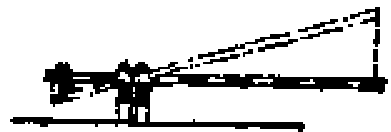
\includegraphics[width=4cm]{../pic/czjh2-ch6-xiti22-01.png}
    \caption*{(第 1 题)}
\end{figure}


\xiaoti{$\triangle ABC$ 中, $AB = 12$ 厘米, $BC = 18$ 厘米, $CA = 24$ 厘米。
    另一个和它相似的 $\triangle A'B'C'$, 周长为 81 厘米。求 $\triangle A'B'C'$  的各边长。
}


\xiaoti{两个相似三角形的一对对应边长分别是 35 厘米和 14 厘米。}
\begin{xiaoxiaotis}

    \xxt{它们的周长相差 60 厘米,求这两个三角形的周长;}

    \xxt{它们的面积相差 588 平方厘米,求这两个三角形的面积。}

\end{xiaoxiaotis}

\xiaoti{$CD$ 是 $Rt \triangle ABC$ 的斜边 $AB$ 上的高。设 $BC = a$、 $CA = b$、
    $AB = c$、 $CD = h$、 $AD = q$、 $DB = p$。
}
\begin{xiaoxiaotis}

    \xxt{已知:$c = 29$, $p = 6$,求 $h$ 和 $b$;}

    \xxt{已知:$a = 5$, $h = 4$,求 $p$ 和 $q$;}

    \xxt{已知:$a = 10$, $p = 6$,求 $q$ 和 $b$;}

    \xxt{已知:$p = 4$, $h = 10$,求 $a$ 和 $b$。}

\end{xiaoxiaotis}


\xiaoti{已知:$\triangle ABC$ 中, $\angle BAC$ 是直角, $AC > AB$, $AD$ 是高, $M$ 是 $BC$ 的中点。\\
    求证: $AC^2 - AB^2 = 2 DM \cdot BC$。
}

\xiaoti{$\triangle ABC$ 中, $\angle BAC$ 是直角, $AD$ 是高, $DE$ 是 $\triangle ABD$ 的高。
    求证: $AD^2 = AC \cdot DE$。
}

\xiaoti{$\triangle ABC$ 中, $\angle BAC$ 是直角, $AD$ 是高。求证:}
\begin{xiaoxiaotis}

    \xxt{如果 $AB = 2 AC$, 那么 $5 AD = 2 BC$;}

    \xxt{如果 $BC = 5 DC$, 那么 $BC^2 = 5 AC^2$。}

\end{xiaoxiaotis}


\xiaoti{如图,矩形 $ABCD$ 中, $AB = a$, $BC = b$, $M$ 是 $BC$ 的中点, $DE \perp AM$, $E$ 是垂足。\\
    求证: $DE = \dfrac{2ab}{\sqrt{4a^2 + b^2}}$。
}

\begin{figure}[htbp]
    \centering
    \begin{minipage}[b]{7cm}
        \centering
        \begin{tikzpicture}
    \tkzDefPoints{0/0/B, 3.2/0/C, 3.2/2/D, 0/2/A}
    \tkzDefMidPoint(B,C)  \tkzGetPoint{M}
    \tkzDefLine[altitude](A,D,M)  \tkzGetPoint{E}

    \tkzDrawPolygon(A,B,C,D)
    \tkzDrawSegments(A,M  D,E)
    \tkzMarkRightAngle(D,E,A)
    \tkzLabelPoints[left](A,B)
    \tkzLabelPoints[right](C,D)
    \tkzLabelPoints[below](M)
    \tkzLabelPoints[below left=-.3em](E)
\end{tikzpicture}


        \caption*{(第 8 题)}
    \end{minipage}
    \qquad
    \begin{minipage}[b]{7cm}
        \centering
        \begin{tikzpicture}
    \tkzDefPoints{0/0/A, 3/0/B, 3.8/2/C, 0.8/2/D}
    \tkzDefPointOnLine[pos=0.6](A,C)  \tkzGetPoint{O}
    \tkzDefLine[parallel=through O](B,C)  \tkzGetPoint{e}
    \tkzInterLL(O,e)(A,B)  \tkzGetPoint{E}
    \tkzDefLine[parallel=through O](A,B)  \tkzGetPoint{f}
    \tkzInterLL(O,f)(A,D)  \tkzGetPoint{F}

    \tkzDrawPolygon(A,B,C,D)
    \tkzDrawSegments(A,C  O,E  O,F)
    \tkzLabelPoints[left](A,D,F)
    \tkzLabelPoints[right](B,C)
    \tkzLabelPoints[below](E)
    \tkzLabelPoints[below right](O)
\end{tikzpicture}


        \caption*{(第 10 题)}
    \end{minipage}
\end{figure}


\xiaoti{在一张比例尺为 $1:50000$ 的地图上,一块多边形地区的周长是 72 cm,面积是 $320\;\pflm$。
    地区的实际周长是多少?面积是多少?
}

\xiaoti{如图,设 $O$ 是四边形 $ABCD$ 的对角线 $AC$ 上的一点, $OF \pingxing CD$、 $OE \pingxing BC$。\\
    求证: $\text{四边形} \; AEOF \xiangsi \text{四边形} \; ABCD$。
}


\xiaoti{已知:四边形 $ABCD$ 和四边形 $A'B'C'D'$ 中, $\angle A = \angle A'$,
    $\dfrac{AB}{A'B'} = \dfrac{BC}{B'C'} = \dfrac{CD}{C'D'} = \dfrac{DA}{D'A'}$。
    求证: $\text{四边形} \; ABCD \xiangsi \text{四边形} \; A'B'C'D'$。
}

\end{enhancedline}
\end{xiaotis}

